\chapter{System Design Description}
The following chapter gives an overview behind the system design of \projectName. The chapter begins by working through the hardware system architecture diagram shown in Figure \ref{IM_SystemArchitecture}. The first consideration is the size and mounting needs of the system, provided by the mechanical platform. This gives a good start to elaborate on the needed capabilities of the proposed method of propulsion. The next considerations are the electronic modules required to run all the necessary peripherals. Finally, to interface all these blocks together will require both software and control architectures. This chapter will discuss the requirements for each section and expand on how the interfacing for the entire system will function.

	\section{System Hardware Architecture}
	The system architecture for \projectName is laid out below in Figure \ref{IM_SystemArchitecture}. The hardware system comprises of 3 main subsystems, namely Mechanical Construction, Propulsion and Electronics. The role each subsystem plays in meeting the system requirements is discussed in more detail below.
	
	\begin{figure}[H]
		\centering
		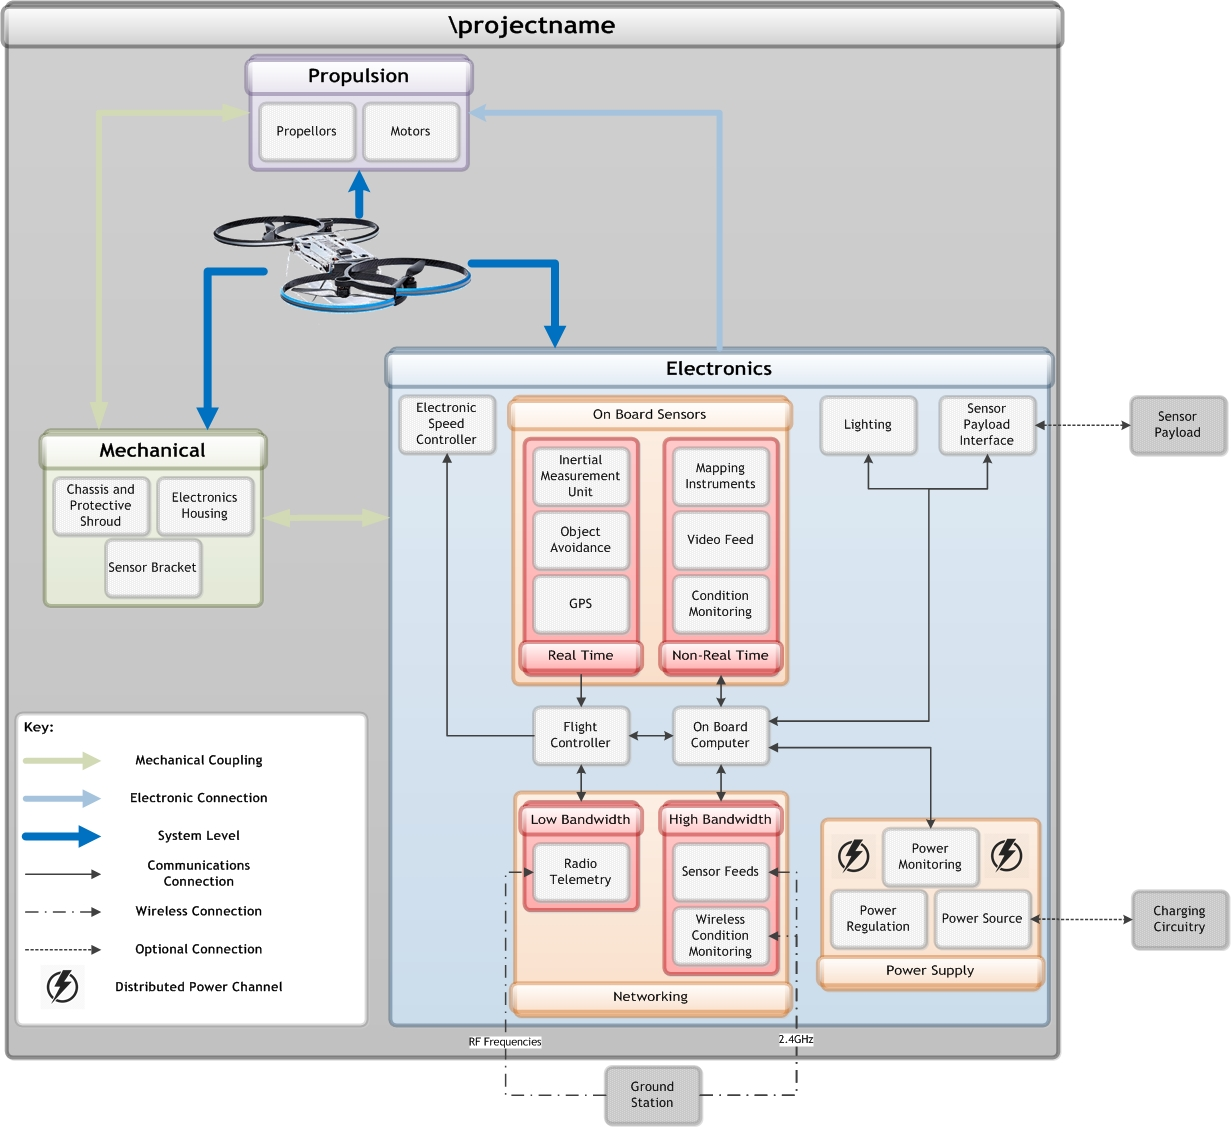
\includegraphics[height = 10cm]{../Design/System/SystemArchitecture/SystemArchitecture.jpg}
		\caption{System Architecture}
		\label{IM_SystemArchitecture}
	\end{figure}
		
		\subsection{Platform Construction}
		The platform is the physical embodiment of the craft. In this context this includes the mechanical construction of the craft, as well as the flight generating components.
		
			\subsubsection{Mechanical Construction}
			The mechanical construction of the system introduces size restrictions for the rest of the system. It should provide adequate mounting for the necessary peripherals described in the sections following. The structure needs to protect the rotors from collisions be means of a shroud and include lightweight landing gear. The chassis must also be such that the weight is distributed as symmetrically as possible. The propulsion system must be housed and provided with rigidity for steady flight control.

			\subsubsection{Propulsion and Flight Characteristics}
			The propulsion system comprises of the motors and propellers. This subsystem needs to supply enough thrust and overhead for steady control, as well as enough lifting capacity to carry any additional, mission sensors. The craft should be able to handle a \payLoadMass payload. To ensure capable disturbance rejection, the total maximum thrust should be no less than $150\%$ of hover.
			
			The craft must efficiently hover and fly at low speeds. The craft should have multiple control surfaces to accurately counter disturbances. Due to the intended use case, the craft will fly with a set orientation and thus does not require the abilities for sharp turns of manoeuvres.
		

		\subsection{Electronics Interface}
		At the core of any reliable robotic platform is a thoroughly planned electronics system, for \projectName this is the most complex subsystem containing the most modules. It is responsible for all intelligence and power generation. This subsection breaks this subsystem into more discrete parts. It begins by separating the two computing modules into real time and non-real time components. The real time components include some of the on board sensors which are required for stable and fast control theories, which all feed into the flight controller. For the drone to successfully navigate an environment it will need to better understand it's surroundings. The flight controller will analyse this data and based on flight software will control the electronic speed controllers. The on board computer will process and handle all non flight critical sensor information and can be considered as the mission computer. The OBC must also have provision to connect to a sensor pack via a predetermined interface. Another useful and necessary function, will be the ability to illuminate a dark area. 
		
		The network design will also consist of 2 discrete wireless links. Each link is dedicated to one of the computing modules. The real time node will be interfaced through a low bandwidth, high range and high reliability interface. With the non-real time node linking to the high bandwidth interface which will have lower range and reliability requirements. Both of these interfaces will link to a ground station of some sort.
		
		No system can operate without a sufficient power source. In the case of any robotic system it is important that every aspect of the design is optimised. To assist with that an electrical analysis is done to help pinpoint some of the major power consuming components. This analysis will also help to evaluate the required power source. The capacity of the power supply is limited by weight and should be optimised to the lifting capacity of the platform. Once the battery chemistry has been decided upon, work can be done to design a robust power management system. Limiting the leakage of every subsystem as well as choosing efficient modules are both part of an effective power management system. To complete the subsystem will require some form of power monitoring as well as an efficient charging scheme.
		
			\subsubsection{Flight Controller}
			The flight controller is responsible for handling all the flight critical sensor data. Using a mixing algorithm it will then output signals to the electronic speed controllers. There are multiple options for flight controllers, all tailored to different applications, platforms and flying styles. Each option has there own level of reconfigurability. For this application it is important that the chosen flight controller allows access to both the inner control loops as well as allows additional sensor data to be added into the architecture. The flight controller is also responsible for handling the pilot commands sent via the radio link, as well as transmitting in flight diagnostic information back to the ground control station.
				
			\subsubsection{Electronic Speed Controller}
			The flight controller will take in information from some of the on board sensors. It then sends a motor control command based on that information to the electronic speed controller (ESC), which directly controls the speed of each motor. This part needs to be chosen based on the maximum amount of current it can handle. At 100\% throttle the current draw of the motor should not exceed 75\% of the ESC's limit. Another important consideration is the ESC's refresh rate and computing speed. The flight controller will be rapidly sending data to the ESC. The quicker the module can respond, the more accurately the platform will fly. 
			
			Each ESC has built in intelligence and will have their own dedicated firmware. Most ESCs will come with built in firmware, which must be tailored for a quadcopter configuration.
			
			\subsubsection{On Board Computer}
			Where the flight controller ensures the craft maintains steady flight, the On Board Computer (OBC) handles all higher level processing. This will include interfacing to the rest of the on board sensors, the sensor pack as well as handling the high bandwidth networking. The OBC should not be required for flight purposes, and can thus be considered as a dedicated mission computer. 
			The OBC should be as light weight as and low power as possible. The OBC must be sufficiently powerful to do real time analysis of camera data. The OBC must have multiple communication ports to easily interface to other sensors.
					
			\subsubsection{Networking}
			This subsystem will handle control commands, flight and diagnostic data or real time sensing information. As described above these have been separated into two distinct categories, low and high bandwidth or alternatively named as high and low range. 
			
				\paragraph{Low Bandwidth, High Range}
				A reliable connection is an important factor to ensure a successful mission the hardware will be validated against it's range, speed, packet loss and ultimately reliability.
						
				The design will incorporate multiple communication peripherals as a fail-safe in case communications are lost to the base station. The pilot needs full control through it and any relevant data that needs to be transmitted will be sent here as well.
						
				\paragraph{High Bandwidth, Low Range}
				The higher bandwidth connection will be used for higher level mission control and data. The high bandwidth link should be able to transmit large streams of data between the craft and the ground control station. 
	
			
			\subsubsection{On Board Sensors}
			
			
			\subsubsection{Sensor Pack}
			The actual sensor pack in question will remain generic. So that the platform can cater for an array of sensing devices and applications. To ensure compatibility, the sensor pack needs to be able to powered as well as communicated to. It will have access to interface directly to the OBC.
	
	
			\subsubsection{Power Supply}
				\subsubsection{Electrical Requirements Analysis}
				\subsubsection{Power Source}
				\subsubsection{Power Regulation}
				\subsubsection{Power Monitoring}
				
	\section{System Software Framework}
	The electronic components gather and collect all the necessary information, the software combines it all and controls the flow of data to obtain stable flight and more. The software system can also be broken down into different operational groups or subsystems. These are, the firmware running the flight controller, the communication protocols used between the software nodes as well as the ground control station. The ground control station although not deployed on the platform, is still mission critical and must be able to display in flight data and send commands to the craft. The last module is the logging and simulation node, which allows for an in depth understanding of untested flight dynamics.
	
		\subsection{Flight Controller Firmware}
		Most commercial flight controllers will come preprogrammed with flight control software. The required firmware blocks are represented in Figure \ref{IM_SoftwareArchitecture} and are discussed in the subsections that follow.
		
		\todo[inline]{Make figure and add in the blocks required}
		\begin{figure}[H]
			\centering
			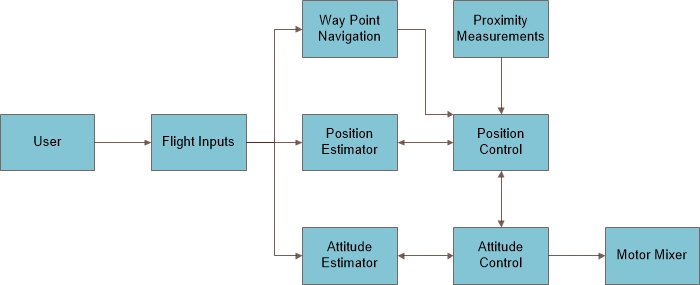
\includegraphics[height = 4cm]{../Design/Software/FirmwareBlocks}
			\caption{Software Framework}
			\label{IM_SoftwareArchitecture}
		\end{figure}
		
			\subsubsection{Flight Modes}
			All the different modules must be accessible and configurable. The flight controller must be able to handle different flight modes that can be changed during a mission. There must be an autonomous flight mode, where the craft can follow set way points. When not in autopilot, the pilot must be able to send the craft commands to control it's movement. 
			
			\subsubsection{Position Controller}
			For precise control, the firmware will need both a well defined position and attitude estimator. 
			The position estimator must accurately predict the current position of the craft and accept new set points based on user defined way points. 
			The position control must create angle and throttle commands to rectify the error calculated in the position estimator. The commands are then sent to the attitude estimator to create new attitude set points. 
			
			\subsubsection{Attitude Controller}
			The attitude estimator must measure the crafts orientation and will be fed information from both the on board positioning monitoring system, as well as the inertial measurement unit. The attitude estimator must be able to take new set points from either the user or the position controller, depending on flight mode. The set points are then fed into the attitude control which calculates the error and generates PWM motor commands that are sent to the ESCs.
			
			\subsubsection{Way Point Navigation}
			As mentioned, the controller must have a way points navigation module, that can feed new position commands into the position estimator. The way points module will need to be able to update during a mission. The way points become the mission goal, to obtain this goal in a confined space, the craft must be able to deviate off course to avoid obstacles. 
			
			\subsubsection{Proximity Sensing}
			Obstacle avoidance calls for a module that can calculate the craft's proximity to it's immediate surroundings. This module will accept information from proximity sensors and output warnings to the position control. The position control must generate a flight strategy that allows for deviations off course, while the total deviation must round to zero.
					
		\subsection{Communication Protocols}
		The communication to and from the craft is represented in \ref{IM_SystemArchitecture}.
			\subsubsection{Radio and Telemetry}
			The radio frequency (RF) must be \todo{insert South African regulation frequency}. This link is a higher range connection and must be able to send commands reliably to the craft. 
			The telemetry link is between the GCS and the craft. It is a higher bandwidth connection and must be able to send in flight data and receive commands from the GCS. More is specified in the ground control software section.
			\subsubsection{Mission Computer}
			\subsubsection{External Sensors}
		\subsection{Ground Control Software}
		The ground station must deploy software that can visualise flight data. The GCS must also be able to send commands to the craft as well as update the mission plan.
			\subsubsection{Data Visualisation}
			\subsubsection{Basic Commands}
			\subsubsection{Way Points}
		\subsection{Logging and Simulation}
		Flight data must be collected and accessible for interpretation and graphing. New strategies can be developed from this data and tested by simulating certain aspects of the hardware.
			\subsubsection{Graphing}
			\subsubsection{Simulation in the Loop}
			\subsubsection{Hardware in the Loop}			
		







